\subsection{Algorithm}

While we have sensor controllers that try to abstract away detail, we realized that this wasn't nearly enough for the NXTCam sensor. Even after sorting out zero-size boxes, max-length bars and boxes that were simply too large, we would still be left with a large amount of erroneous measurements that would be really tough to identify as faulty.

Multiple measurements and statistical analysis of their placement might get us halfway there, but we concluded it to be safer to build an algorithm for staying within a lane that was resistant against singular faulty measurements.

We experimented with other approaches, but we had the most success with a reactionary algorithm that made incremental changes to the turning angle that it suggested the bus should drive. 

As such, we made ???


It detects which objects it is on collision course with, and corrects based on the one it's going to hit first. 

\todo{Finish this chapter and add in a piece of the code to examine. Delete the rest.}






\todo{We have a new Algorithm that does something else. This subsection needs to be re-written.}
In this section the algorithm that ensures that the bus always stays within the road lane is described. 

The intent for the algorithm is to calculate an optimal line that the bus should follow in order to keep within lane markings. Using this result, it will call the Driving-component and inform it how much the bus should turn its wheels and for how long with it's current speed. 

Before the points gained through the NxtCamLineTrackController can be used, they need to be sorted in left and right side. After this we calculate a bézier curve\todo{We dont juse this anymore} for each side to find a smooth midpoint line for the bus to follow. This is not quite as simple as it seems, as we need to handle the cases where the line tracker returns only very few points. For instance, if it returns only one coordinate for the left lane marking, then we cannot calculate a proper curve without knowledge of where at least one previous coordinate in the left lane was placed. 

To solve this, we save old measurements from the last time we calculated the path for the bus. However, these need to be moved along the x or y-axis to fit with the new position of the bus compared to the place where the old measurement took place. Additionally, these measurement will need to be rotated if the bus has driven part of a road curve since the last measurement. Also the bus will need to handle the case where there are zero measurement in the side. This is done by taking the measured point which is the farthest away, and the point previous to that in the same side. Next these two points are used to make a right-angle triangle so the farthest away point of the other side can be calculated, see figure \ref{fig:findK}. By doing this we get the point farthest away the camera can see in both sides. Now the bézier curves for both side will show approximately same length of the road. And that will make our calculation of midpoints between the two curves more accurate since the amount of points calculated on each bézier curves is a constant.

Now a constant of midpoints is calculated and the slope and length between each point is found. The slope tells the angle the bus needs to turn, if the slope is negative it means turn left, if positive turn right. And the length is the distance to be driven with the found slope. 


\begin{figure}[ht]
    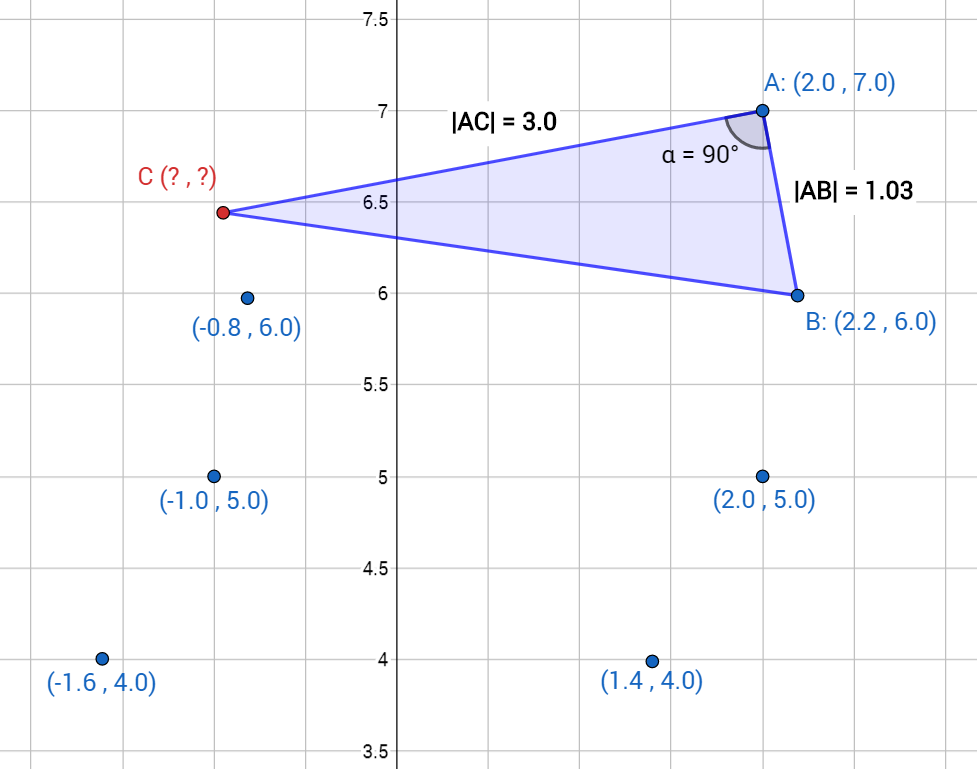
\includegraphics[width=\textwidth]{Images/Design/findK.PNG}
    \caption{Balance left/right data length.\todo[inline]{We need a better description of what is going on in this Figure. Do we even use the figure for anything now?}}
    \label{fig:findK}
\end{figure}




\begin{algorithm}[H]
 \KwData{this text}
 \KwResult{how to write algorithm with \LaTeX2e }
 initialization\;
 \While{not at end of this document}{
  read current\;
  \eIf{understand}{
   go to next section\;
   current section becomes this one\;
   }{
   go back to the beginning of current section\;
  }
 }
 \caption{How to write algorithms}
\end{algorithm}







\todo{Add the pictures I created for pineTreeProblem and lane correction over time}\todo{This is made according to the old ways. It needs to be changed to the new ways that we implement it.}
%I feel like making the nxtCamLineTrack just return third order polynomials would have been better.

\begin{description}
    \item[NxtCamLineTrackController: Track Lines]
    Gets the cleaned coordinates from a picture using the previously described NxtCamLineTrackController class. 
    \item[Combine Old And New Coordinates]
    Combines old and new coordinates, moving and rotating the measurements to fit with the new position and wheel angle of the bus. 
    \item[Sort Data]
    Splits the coordinates into measurements belonging to the left and the right lane marking. 
    \item[Bézier Curve Calculation]\todo{Remove this part since it is no longer relevant?}
    A bézier curve is calculated for the left and right lane markings. Using this, a number of points in the middle of the road between the two bézier curves is calculated.
    \item[Calculate Driving Direction]
    Calculates which direction the bus should turn optimally. 
    \item[Call Driving Component]
    Calls the driving and informs it of the results.
\end{description}
\todo{1. LoadData, 2. Update Data to global space, 3. Sort New Data y and side, 4. Update OldData, 5. Combine Old and New data, 6. BezierCurves, 7. MidPoints, 8. Slope/Length.}

This algorithm has been implemented in the StayWithinLane-class of the program. \todo{We're in design, Can't write this!}
\todo{Describe part of code?}


%() Stay Within Lines: Algoritme ()- Basically, den kører prik-til-prik med midtpunkter
%	(Punkter på koordinatsystem) NxtCamV4 Line Tracking Driver: Track Line ()
%	(Gamle + Nye punkter på koordinatsystem) Sammensæt gammelt og nyt data ([Nye] Punter på koordinatsystem, Bus Point, [Gammel] Midpoint Bezier Curve)
%	(Sorteret Data Venstre, Sorteret Data Højre) Sorter Data (Gamle + Nye punkter på koordinatsystem)
%	(0-8 Midtpoints) Bezier Curve Udregning (Sorteret Data Venstre, Sorteret Data Højre)
%	*(Grader rotation, afstand der skal køres) Regn kørselsrute (0-8 Midtpoints)					- Hvis bussen ikke er i midten, skal den køre hen mod midtpoint. Håndterer også hvis den ikke får nok/nogle punkter